\documentclass{Numerieke}
\newcommand\inv[1]{#1\raisebox{0.8ex}{$\scriptscriptstyle\!*$}}
\newcommand\transpose[1]{#1\raisebox{0.8ex}{$\scriptscriptstyle\!T$}}
\newcommand\totdeK[1]{#1\raisebox{0.8ex}{$\scriptscriptstyle\!(k)$}}

%==PACKAGES==%
\usepackage[dutch]{babel}
\usepackage{graphicx}
\usepackage{float}
\usepackage{amsmath}
\usepackage{mathtools}
\usepackage[table,xcdraw]{xcolor}
\usepackage[normalem]{ulem}
\useunder{\uline}{\ul}{}
\graphicspath{{pictures/}}

\begin{document}
% == TITELPAGINA == %
%\input(nmbvoorblad)

%TEMP frontpage
\title{Numerieke Modellering en Benadering}
\maketitle

\section{QR factorisatie en kleinste kwadraten problemen}
\subsection{Opgave 1}

\newline
\textbf{1.A: Eigenwaarden en eigenvectoren} \newline
De vector $\vec{v}$ is een eigenvector van de vierkante matrix A \textit{(n$\times$n)} indien volgende vergelijking geldt:
 \[A\vec{v} = \lambda\vec{v}\] 
 Met $\lambda$  de bijhorende eigenwaarde en een natuurlijk getal.\newline 
 \newline
 \textit{Stelling:} \newline
 De Householder transformatie matrix F is orthogonaal en symmetrisch met enkel reeële waarden. \newline
 \textit{Bewijs: } \newline
 \textbf{F is symmetrisch} \newline
 \textit{Defenitie :} \(F=I-2\frac{v\inv{v}}{\inv{v}v}  \)
 \newline
 Met de genormaliseerde vector \(w = \frac{v}{\inv{v}v}\) is de defenitie herschrijfbaar als: 
 \[F=I-2w\inv{w}\]
 Aangezien de beide termen symmetrisch zijn is de householder transformatiematrix zelf ook symmetrisch.\newline
 \textbf{F is orthogonaal} \newline
 Indien \transpose{F}F=I zal F orthogonaal zijn.
 \[\transpose{F}F = \transpose{(I-2w\transpose{w})}(I-2w\transpose{w}) = (I-4w\transpose{w}+4w\transpose{w}w\transpose{w}) = I\]
 Hierbij is \transpose{w}w = 1 aangezien w genormaliseerd is. Daardoor wordt de vergelijking herleid tot : \newline
  \[\transpose{F}F = (I-4w\transpose{w}+4w\transpose{w}) = I\]
  \newline
 Aangezien F orthogonaal is, hebben de eigenwaarden een absolute waarde van 1 omdat de vermenigvuldiging met een orthogonale matrix een isometrie is.\newline
  F is symmetrisch en reeël dus alle eigenwaarden zullen reeël zijn. Daardoor kunnen de eigenwaarden kunnen herleidt worden tot 1 en -1.
  \newline
  Aangezien \(Fw = w-2w(\transpose{w}w)=-w}\) is minstens er één eigenwaarde -1 en voor alle vectoren u, loodrecht op w, geldt:  \(Fu = u-0w=u}\)
\newline
\newpage
\textbf{1.B: Geometrische interpretatie} \newline
\begin{figure}[H]
	\caption{Eigenwaarden en vectoren van de Householdertransformatiematrix}
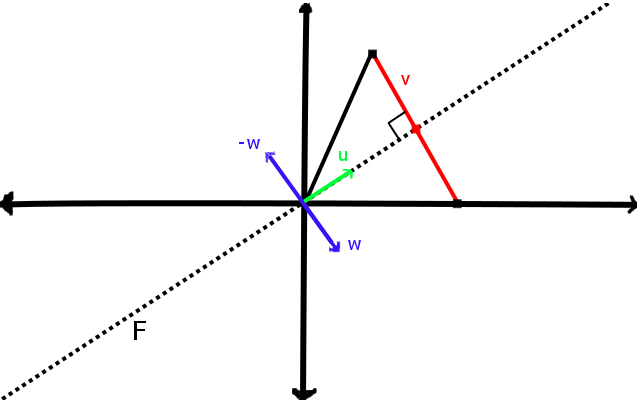
\includegraphics[scale=0.3]{Householdereigenwaarden.png}
\centering
\end{figure}
Zoals te zien is op de figuur zal de Householder functie de genormaliseerde vector w projecteren op -w omdat F een isometrie is. Daarnaast zullen alle loodrechte vectoren op w op F liggen en zals er geprojecteerd worden op hetzelfde punt.

\subsection{Opgave 2}
\textbf{2.B: Vergelijking resultaten}
% Please add the following required packages to your document preamble:
% \usepackage[table,xcdraw]{xcolor}
% If you use beamer only pass "xcolor=table" option, i.e. \documentclass[xcolor=table]{beamer}
% \usepackage[normalem]{ulem}
% \useunder{\uline}{\ul}{}
\begin{table}[H]
	\centering
	\caption{Conditie van A gelijk aan 1}
	\label{my-label}
	\begin{tabular}{l|
			>{\columncolor[HTML]{EFEFEF}}l 
			>{\columncolor[HTML]{EFEFEF}}l 
			>{\columncolor[HTML]{EFEFEF}}l 
			>{\columncolor[HTML]{EFEFEF}}l 
			>{\columncolor[HTML]{EFEFEF}}l 
			>{\columncolor[HTML]{EFEFEF}}l 
			>{\columncolor[HTML]{EFEFEF}}l 
			>{\columncolor[HTML]{EFEFEF}}l }
		\cline{2-9}
		\multicolumn{1}{c|}{{\ul \textbf{}}}               & \multicolumn{4}{c|}{\cellcolor[HTML]{C0C0C0}{\ul \textbf{Explicit}}}                                                                                                                                                                 & \multicolumn{4}{c|}{\cellcolor[HTML]{C0C0C0}{\ul \textbf{Implicit}}}                                                                                                                                                                 \\ \hline
		\multicolumn{1}{|l|}{\cellcolor[HTML]{C0C0C0}n}    & \multicolumn{1}{l|}{\cellcolor[HTML]{EFEFEF}\delta x} & \multicolumn{1}{l|}{\cellcolor[HTML]{EFEFEF}r} & \multicolumn{1}{l|}{\cellcolor[HTML]{EFEFEF}\delta x/x} & \multicolumn{1}{l|}{\cellcolor[HTML]{EFEFEF}K(A)r/b} & \multicolumn{1}{l|}{\cellcolor[HTML]{EFEFEF}\delta x} & \multicolumn{1}{l|}{\cellcolor[HTML]{EFEFEF}r} & \multicolumn{1}{l|}{\cellcolor[HTML]{EFEFEF}\delta x/x} & \multicolumn{1}{l|}{\cellcolor[HTML]{EFEFEF}K(A)r/b} \\ \hline
	\multicolumn{1}{|l|}{\cellcolor[HTML]{C0C0C0}10}   & 6.9162e-16                                          & 6.2979e-16                                         & 4.1395e-16                                                & 3.7762e-16                                                    & 5.9923e-16                                          & 6.5433e-16                                         & 3.6326e-16                                                & 3.9842e-16                                                    \\ \cline{1-1}
	\multicolumn{1}{|l|}{\cellcolor[HTML]{C0C0C0}100}  & 1.5897e-14                                          & 1.6162e-14                                         & 3.0763e-15                                                & 3.099e-15                                                     & 6.4763e-15                                          & 6.3391e-15                                         & 1.3988e-15                                                & 1.3992e-15                                                    \\ \cline{1-1}
	\multicolumn{1}{|l|}{\cellcolor[HTML]{C0C0C0}1000} & 2.6441e-13                                          & 2.6477e-13                                         & 1.6695e-14                                                & 1.6723e-14                                                    & 4.9441e-14                                          & 4.93e-14                                           & 3.7536e-15                                                & 3.7537e-15                                                    \\ \cline{1-1}
\end{tabular}
\end{table}
 \begin{table}[H]
 	\centering
 	\caption{Conditie van A gelijk aan 10^4}
 	\label{my-label}
 	\begin{tabular}{l|
 			>{\columncolor[HTML]{EFEFEF}}l 
 			>{\columncolor[HTML]{EFEFEF}}l 
 			>{\columncolor[HTML]{EFEFEF}}l 
 			>{\columncolor[HTML]{EFEFEF}}l 
 			>{\columncolor[HTML]{EFEFEF}}l 
 			>{\columncolor[HTML]{EFEFEF}}l 
 			>{\columncolor[HTML]{EFEFEF}}l 
 			>{\columncolor[HTML]{EFEFEF}}l }
 		\cline{2-9}
 		\multicolumn{1}{c|}{{\ul \textbf{}}}               & \multicolumn{4}{c|}{\cellcolor[HTML]{C0C0C0}{\ul \textbf{Explicit}}}                                                                                                                                                                 & \multicolumn{4}{c|}{\cellcolor[HTML]{C0C0C0}{\ul \textbf{Implicit}}}                                                                                                                                                                 \\ \hline
 		\multicolumn{1}{|l|}{\cellcolor[HTML]{C0C0C0}n}    & \multicolumn{1}{l|}{\cellcolor[HTML]{EFEFEF}\delta x} & \multicolumn{1}{l|}{\cellcolor[HTML]{EFEFEF}r} & \multicolumn{1}{l|}{\cellcolor[HTML]{EFEFEF}\delta x/x} & \multicolumn{1}{l|}{\cellcolor[HTML]{EFEFEF}K(A)r/b} & \multicolumn{1}{l|}{\cellcolor[HTML]{EFEFEF}\delta x} & \multicolumn{1}{l|}{\cellcolor[HTML]{EFEFEF}r} & \multicolumn{1}{l|}{\cellcolor[HTML]{EFEFEF}\delta x/x} & \multicolumn{1}{l|}{\cellcolor[HTML]{EFEFEF}K(A)r/b} \\ \hline
	 	\multicolumn{1}{|l|}{\cellcolor[HTML]{C0C0C0}10}   & 3.0736e-12                                          & 6.4259e-12                                         & 1.8003e-12                                                & 4.5603e-12                                                    & 1.722e-12                                           & 3.3718e-12                                         & 1.0098e-12                                                & 2.3895e-12                                                    \\ \cline{1-1}
	 	\multicolumn{1}{|l|}{\cellcolor[HTML]{C0C0C0}100}  & 9.2189e-11                                          & 9.7262e-11                                         & 1.6467e-11                                                & 2.2014e-11                                                    & 1.8454e-11                                          & 2.7045e-11                                         & 3.7652e-12                                                & 6.9365e-12                                                    \\ \cline{1-1}
	 	\multicolumn{1}{|l|}{\cellcolor[HTML]{C0C0C0}1000} & 1.5252e-09                                          & 1.533e-09                                          & 9.5391e-11                                                & 1.1298e-10                                                    & 1.6481e-10                                          & 1.7583e-10                                         & 1.1824e-11                                                & 1.636e-11                                                     \\ \cline{1-1}
	 \end{tabular}
 \end{table}
 \begin{table}[H]
 	\centering
 	\caption{Conditie van A gelijk aan 10^8}
 	\label{my-label}
 	\begin{tabular}{l|
 			>{\columncolor[HTML]{EFEFEF}}l 
 			>{\columncolor[HTML]{EFEFEF}}l 
 			>{\columncolor[HTML]{EFEFEF}}l 
 			>{\columncolor[HTML]{EFEFEF}}l 
 			>{\columncolor[HTML]{EFEFEF}}l 
 			>{\columncolor[HTML]{EFEFEF}}l 
 			>{\columncolor[HTML]{EFEFEF}}l 
 			>{\columncolor[HTML]{EFEFEF}}l }
 		\cline{2-9}
 		\multicolumn{1}{c|}{{\ul \textbf{}}}               & \multicolumn{4}{c|}{\cellcolor[HTML]{C0C0C0}{\ul \textbf{Explicit}}}                                                                                                                                                                 & \multicolumn{4}{c|}{\cellcolor[HTML]{C0C0C0}{\ul \textbf{Implicit}}}                                                                                                                                                                 \\ \hline
 		\multicolumn{1}{|l|}{\cellcolor[HTML]{C0C0C0}n}    & \multicolumn{1}{l|}{\cellcolor[HTML]{EFEFEF}\delta x} & \multicolumn{1}{l|}{\cellcolor[HTML]{EFEFEF}r} & \multicolumn{1}{l|}{\cellcolor[HTML]{EFEFEF}\delta x/x} & \multicolumn{1}{l|}{\cellcolor[HTML]{EFEFEF}K(A)r/b} & \multicolumn{1}{l|}{\cellcolor[HTML]{EFEFEF}\delta x} & \multicolumn{1}{l|}{\cellcolor[HTML]{EFEFEF}r} & \multicolumn{1}{l|}{\cellcolor[HTML]{EFEFEF}\delta x/x} & \multicolumn{1}{l|}{\cellcolor[HTML]{EFEFEF}K(A)r/b} \\ \hline
		\multicolumn{1}{|l|}{\cellcolor[HTML]{C0C0C0}10}   & 2.7567e-08                                          & 4.432e-08                                              & 1.6671e-08                                                & 3.499e-08                                                     & 1.6694e-08                                          & 2.4974e-08                                             & 9.8794e-09                                                & 1.785e-08                                                     \\ \cline{1-1}
		\multicolumn{1}{|l|}{\cellcolor[HTML]{C0C0C0}100}  & 8.0343e-07                                          & 8.27904e-07                                            & 1.5567e-07                                                & 1.9718e-07                                                    & 1.4431e-07                                          & 1.78499e-07                                            & 3.2706e-08                                                & 4.9677e-08                                                  \\ \cline{1-1}
		\multicolumn{1}{|l|}{\cellcolor[HTML]{C0C0C0}1000} & 1.533e-05                                           & 1.542e-05                                         & 9.5357e-07                                                & 1.1203e-06                                                    & 1.526e-06                                           & 1.6375e-06                                           & 1.086e-07                                                 & 1.4195e-07                                                    \\ \cline{1-1}
	\end{tabular}
\end{table}

Bij het vergelijken van de impliciete en expliciete methoden voor matrices van dezelfde grootte is er een klein verschil in nauwkeurigheid. De Impliciete functie zal iets nauwkeuriger zijn omdat het de matrix Q zelf niet meer moet samenstellen en zo minder onderhevig zijn aan afrondingsfouten. Verder is het zichtbaar dat voor alle conditiegetallen van A de nauwkeurigheid van de resultaten zal dalen naarmate de grootte van A toeneemt. Dit komt omdat er meer elementen van x berekend moeten worden en daardoor meer fouten in het algoritme kunnen voorkomen. \newline Bij het toenemen van het conditiegetal van de matrix zien we ook een verlies in beduidende cijfers gelijk aan k (= 4). K is hierbij gelijk aan de macht van 10 $(10^k)$ bij het verschil van de huidige en vorige conditie. Dit komt omdat de matrix steeds slechter geconditioneerd is en zo meer beduidende cijfers verliest aan fouten. \newline 
De scherpte van de grens blijft ongeveer hetzelfde voor de verschillende condities van A.  
\begin{figure}[H]
	\caption{Uitvoeringstijd: Expliciet(rood), Impliciet(Blauw) }
	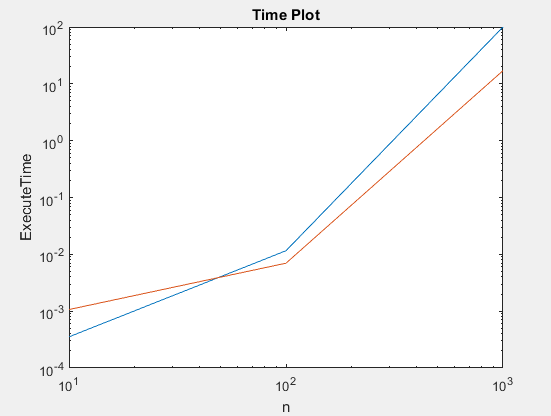
\includegraphics[scale=0.6]{HouseholderTimePlot.png}
	\centering
\end{figure}
\newline
In het algemeen geval zou de impliciete versie sneller moeten zijn als de expliciete versie. In opdracht 2 is dit enkel niet het geval bij de kleine matrix. Dit komt omdat we bij de impliciete versie de matrix Q niet expliciet moeten opstellen en zo geen overbodige tijd verliezen. Verder heeft de conditie van de matrix geen invloed op de uitvoeringstijd van beide algoritmes. 

\subsection{Opgave 3}
Met behulp van de QR factorisatie is het mogelijk om een kleinste kwadraten probleem op te lossen. De projector \(P=Q\inv{Q}\) projecteert de vector b in de range van A en zo is het mogelijk om een exacte oplossing van x te vinden voor \(QRx=Q\inv{Q}\). Dit zal dan herleidt worden tot \(Rx=Qb\) en zal de uitkomst zo dicht mogelijk bij de waarden van b liggen. 
\begin{figure}[H]
	\centering
	\caption{Vergelijking tijdsvertragingen}
	\begin{minipage}[l]{.3\textwidth}
		\centering
		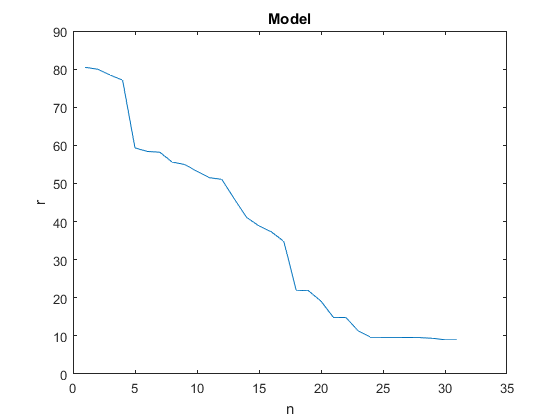
\includegraphics[width=1.05\linewidth]{Model_opgave3}
		\captionof{Residu model}
		\label{fig:test1}
	\end{minipage}%
	\begin{minipage}[r]{.3\textwidth}
		\centering
		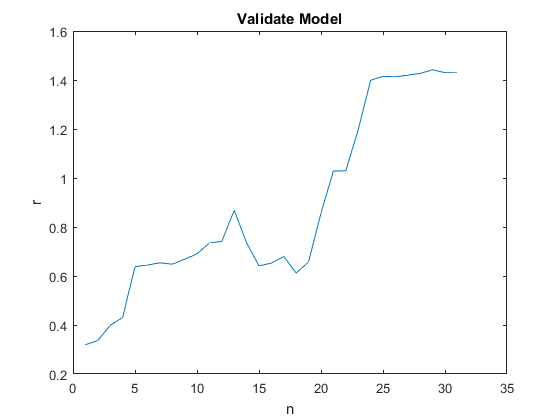
\includegraphics[width=1.05\linewidth]{Validate_model_opgave3}
		\captionof{Residu validate model}
		\label{fig:test2}
	\end{minipage}
\end{figure}
Voor de beide data is het residu het kleinste voor een grotere n. De winst in nauwkeurigheid verloopt tevens trager naarmate n groter wordt. Een voldoende hoge n zal een geschikte keuze zijn voor dit probleem.
\newpage
\section{Iteratieve methoden}
\subsection{Opgave 4}
\textbf{4.A: Rayleigh quotiënt van A \in$ [\lambda\textsubscript{min},\lambda\textsubscript{max}]$} \newline
Definitie Rayleigh quotiënt voor matrix A : $\(r(x) = \frac{\transpose{x}Ax}{\transpose{x}x}$\) met $x\neq0$. \newline
Gebruik makend van de eigenwaardendecompositie van de matrix A = U$\Lambda\inv{U}$ is de teller te schrijven als $\(\transpose{x}U\Lambda\inv{U}x =\sum_{i=1}^{n} \lambda_i(u_ix)^2$\) en gelijkaardig is de noemer te schrijven als  $\(\transpose{x}x =\sum_{i=1}^{n}(u_ix)^2 $\).\newline
\newline
Veronderstel nu dat $\(\lambda_1 \geq \lambda_2 \geq ... \geq \lambda_n$\) en hieruit volgt:\newline \[ \lambda_1\sum_{i=1}^{n} (u_ix)^2 \geq \sum_{i=1}^{n} (u_ix)^2 \geq \lambda_n\sum_{i=1}^{n}(u_ix)^2 \] \newline
Gedeeld door de noemer van de aangepaste Rayleigh quotient volgt:
\[ \lambda_1\geq r(x) \geq \lambda_n , r(x)\in [\lambda\textsubscript{min},\lambda\textsubscript{max}] , x\neq0 \]
De extremen $\lambda\textsubscript{1}$ en $\lambda\textsubscript{n}$ worden respectievelijk bereikt voor $x=u\textsubscript{1}$ en $x=u\textsubscript{n}.$
\newline
\newline
\textbf{4.B: Elke waarde van $[\lambda\textsubscript{min},\lambda\textsubscript{max}]$ kan geschreven worden door een Rayleigh quotient}
Aangezien de Rayleigh quotiënt een continue functie is op de eenheids cirkel met $\left\vert|x|\vert\right= 1$ met de stationaire punten de genormaliseerde eigenvectoren van A zoals te zien is op fig 27.1 uit het handboek. Zo zal er voor elke waarde $\lambda_i$ een Rayleigh quotiënt te vinden zijn met: $\lambda_1 = max(r(x))$ en $\lambda_n = min(r(x))$.
\subsection{Opgave 5}
\textbf{5.A}: \newline
\textbf{Rayleigh quotiënt iteratie:} De Rayleigh quotiënt iteratie maakt gebruik van de inverse iteratie en de Rayleigh quotiënt om eigenwaardes en eigenvectoren te bekomen. Het idee is om de eigenwaarde steeds beter te benaderen met de Rayleigh quotiënt om de convergentie van de inverse iteratie te verbeteren. Zo zal de iteratie het aantal juiste cijfers steeds verdriedubbelen. Met deze methode is het mogelijk om de eigenwaarde van de eigenvector die het dichts bij de initieël geschatte eigenvector te vinden. \newline
\textbf{Gelijktijdige iteratie:} De gelijktijdige iteratie maakt gebruik van de \textit{Power iteration} op meerdere vectoren tegelijk. Hiervan kan men dan de QR factorisatie van nemen en zullen de kolomen van Q convergeren naar de eigenvectoren van A. Door de berekening van $\(A^{(k)} = \transpose{(Q^{(k)})}AQ^{(k)}$\) kan men dan de eigenwaardes vinden op de diagonaal van \(A^{(k)}\).\newline
\textbf{QR algoritme zonder shifts:} Het QR algoritme zonder shift gebruikt de QR factoristatie van \(A^{(k-1)} = Q^{(k)}R^{(k)}\) en gaat hierbij steeds \(A^{(k)} = R^{(k)}Q^{(k)}\) bij opstellen. Deze tussenstappen zullen dezelfde waardes geven als de gelijktijdige iteratie als men kan stellen dat \(A^{(k)} = \transpose{(Q^{(k)})}AQ^{(k)} =\transpose{(Q^{(k)})}A^{(k-1)}Q^{(k)} \) omdat \(R^{(k)} = \transpose{(Q^{(k)})}A^{(k-1)}\). Dit wordt bewezen op pagina 217 van het handboek. Deze methoden zal alle eigenwaarden/eigenvectoren terug geven van de matrix A. \newline
\textbf{QR algoritme met shifts:} Het QR algoritme met shifts is gelijkaardig aan het algoritme zonder shift maar door het introduceren van de shift $A \rightarrow A - \mu I$ zal de convergentie kubisch verlopen. De $ \mu $ is hier gelijk aan de Rayleigh quotiënt van de laatste kolom van $Q^{(k)}$. Het algoritme zelf gebruikt de diagonaal elementen van A om te shiften. Dit algoritme zal alle eigenwaarden/eigenvectoren terug geven.
\newpage
\textbf{5.B:}
\textit{“Het convergentiegedrag van het QR-algoritme met Rayleigh quotiënt shift kan gezien worden als een combinatie van dat van de gelijktijdige iteratie en de Rayleigh quotiënt iteratie.”} \newline
\newline
Door het bekijken van de fout over het verloop van de iteraties is het mogelijk de nauwkeurigheid van de algoritmes afzonderlijk te bekijken. Hierop te zien is dat het de QR algoritme met Rayleigh shift zeer snel (al na 1 iteratie) convergeert naar de hoogste precisie en daarna stabiel blijft. De Rayleigh quotiënt convergeert snel en blijft ook stabiel naarmate het aantal iteraties verhoogt. De gelijktijdige iteratie convergeert trager en zal rond de precisie van de Rayleigh quotiënt iteratie blijven alterneren met als ondergrens de precisie van het QR algoritme.\newline
\begin{figure}[H]
	\caption{Nauwkeurigheid: Qr algoritme, Gelijktijdige iteratie en Rayleigh quotiënt op mat1}
	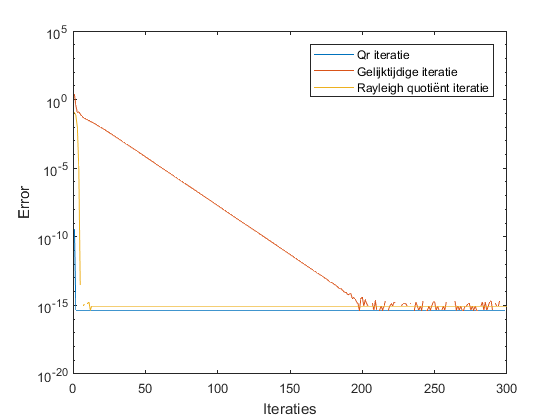
\includegraphics[scale=0.8]{Opgave5b.png}
	\centering
\end{figure}
Door te werken met de geshifte matrix $A \rightarrow A - \mu I$ gaat het QR algoritme eenzelfde voordelig effect als de gelijktijdige iteratie en de inverse iteratie process bekomen. Daardoor zal de ondergrens van de nauwkeurigheid van de gelijktijdige iteratie bij de nauwkeurigheid van de QR iteratie liggen. Dit is zichtbaar door de stappen van het QR algoritme te bekijken. \[A^{(k-1)} - \mu^{(k)}I = Q^{(k)}R^{(k)}\] \[A^{(k)} = R^{(k)}Q^{(k)} + \mu^{(k)}I\] Deze kunnen we dan omvormen tot $\(A^{(k)} = \transpose{(Q^{(k)})}A^{(k-1)}Q^{(k)}$\) \newline en door inductie volgt: \[A^{(k)} = \transpose{(Q^{(k)})}AQ^{(k)}\]Nu moeten we nog een nieuwe vergelijking voor de QR factorisatie opstellen die gelijk is aan : \((A-\mu^{(k)}I)(A-\mu^{(k-1)}I)...(A-\mu^{(1)}I)=Q^{(k)}R^{(k)}\)
Die dan eigenlijk een geshifte variatie is op de gelijktijdige iteratie. Met de shifts gelijk aan de Rayleigh quotiënten van de Rayleigh quotiënt iteratie en zo zal de convergentie van het QR algoritme met shift een combinatie zijn van de gelijktijdige iteratie en de Rayleigh Quotiënt iteratie.



\end{document}